\documentclass[10pt]{article}
\usepackage[polish]{babel}
\usepackage[utf8]{inputenc}
\usepackage[T1]{fontenc}
\usepackage{amsmath}
\usepackage{amsfonts}
\usepackage{amssymb}
\usepackage[version=4]{mhchem}
\usepackage{stmaryrd}
\usepackage{graphicx}
\usepackage[export]{adjustbox}
\graphicspath{ {./images/} }
\usepackage{hyperref}
\hypersetup{colorlinks=true, linkcolor=blue, filecolor=magenta, urlcolor=cyan,}
\urlstyle{same}

\title{GIMNAZJUM }

\author{}
\date{}


\newcommand\Varangle{\mathop{{<\!\!\!\!\!\text{\small)}}\:}\nolimits}

%New command to display footnote whose markers will always be hidden
\let\svthefootnote\thefootnote
\newcommand\blfootnotetext[1]{%
  \let\thefootnote\relax\footnote{#1}%
  \addtocounter{footnote}{-1}%
  \let\thefootnote\svthefootnote%
}

%Overriding the \footnotetext command to hide the marker if its value is `0`
\let\svfootnotetext\footnotetext
\renewcommand\footnotetext[2][?]{%
  \if\relax#1\relax%
    \ifnum\value{footnote}=0\blfootnotetext{#2}\else\svfootnotetext{#2}\fi%
  \else%
    \if?#1\ifnum\value{footnote}=0\blfootnotetext{#2}\else\svfootnotetext{#2}\fi%
    \else\svfootnotetext[#1]{#2}\fi%
  \fi
}

\begin{document}
\maketitle
\begin{enumerate}
  \item Czworokąt wypukły \(A B C D\) ma pole równe 1 . Punkt \(K\) jest symetryczny do punktu \(B\) względem punktu \(A\), punkt \(L\) jest symetryczny do punktu \(C\) względem punktu \(B\), punkt \(M\) jest symetryczny do punktu \(D\) względem punktu \(C\), punkt \(N\) jest symetryczny do punktu \(A\) względem punktu \(D\). Oblicz pole czworokąta KLMN.
  \item Liczby \(a, b, c\) są dodatnie. Wykaż, że
\end{enumerate}

\[
\frac{a}{a+1}+\frac{b}{(a+1)(b+1)}+\frac{c}{(a+1)(b+1)(c+1)}<1
\]

\begin{enumerate}
  \setcounter{enumi}{2}
  \item Okrąg o promieniu 1 jest wpisany w czworokąt wypukły \(A B C D\). Okrąg ten jest styczny do boków \(A B, B C, C D, D A\) odpowiednio w punktach \(K, L, M\), Wiadomo, że
\end{enumerate}

\[
\Varangle K L M=4 \Varangle A K N \quad \text { oraz } \quad \Varangle K N M=4 \Varangle B K L .
\]

Oblicz długość odcinka \(L N\).

\section*{LICEUM}
\begin{enumerate}
  \item Dana jest liczba ośmiocyfrowa \(a\). Liczba ośmiocyfrowa \(b\) powstaje z liczby \(a\) poprzez przestawienie cyfry jedności liczby \(a\) na początek. Wykaż, że jeśli liczba \(a\) jest podzielna przez 101, to liczba \(b\) jest także podzielna przez 101.
  \item Dany jest czworokąt wypukły \(A B C D\), w którym\\
\(\Varangle D A B=\Varangle A B C\). Symetralne odcinków \(A D\) i \(B C\) przecinają się w punkcie \(M\) leżącym na odcinku \(A B\). Udowodnić, że \(A C=B D\).
  \item Punkt \(O\) jest środkiem okręgu opisanego na trójkącie \(A B C\). Punkt \(D\) jest rzutem prostokątnym punktu \(C\) na prosta \(A B\). Wykazać, że \(\Varangle A C D=\Varangle B C O\).\\
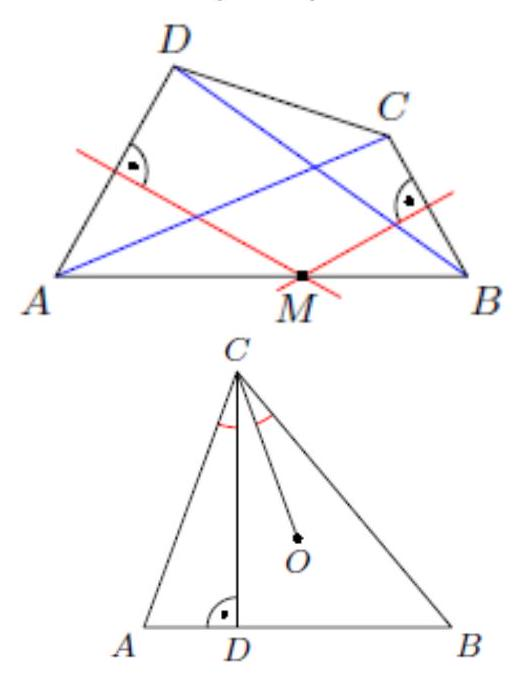
\includegraphics[max width=\textwidth, center]{2024_11_21_eb6613ef93f6a4400caag-1}
\end{enumerate}

\footnotetext{Rozwiazzania należy oddać do piątku 8 kwietnia do godziny 10.35 koordynatorowi konkursu panu Jarostawowi Szczepaniakowi lub swojemu nauczycielowi matematyki lub przestać na adres \href{mailto:jareksz@interia.pl}{jareksz@interia.pl} do piatku 8 kwietnia do pótnocy.
}
\end{document}